
\section{Les signaux OFDM}
\label{sec:defofdm}
\definition{OFDM}{\og L’OFDM (orthogonal frequency-division multiplexing) est un
  procédé de codage de signaux numériques par répartition en fréquences
  orthogonales sous forme de multiples sous-porteuses\fg{}}

Le principe d'un signal OFDM est de répartir notre signal numérique sur de
multiple sous-porteuses orthogonales. Puisque les sous-porteuses sont
orthogonales, en principe elles n'interfèrent pas entre elles. Il est donc
possible d'en extraire l'information facilement\footnote{En pratique, ce n'est
  pas le cas. Ce problème est abordé à la page \pageref{sec:ICI}}. De plus,
puisque le signal numérique est réparti sur plusieurs sous-porteuses on augmente
le débit en transmettant plusieurs état en même temps. La figure
\ref{fig:tempsFreq} illustre la représentation temps-fréquence d'un signal OFDM.

\begin{figure}[!h]
  \centering
  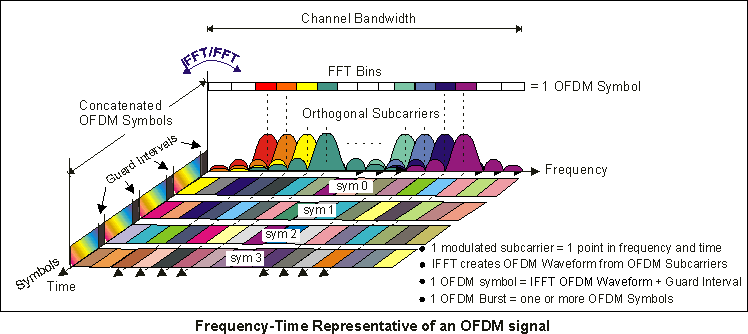
\includegraphics[width=\textwidth]{Frequence_time.png}
  \caption[Temps-Frequence]{Temps-Frequence: representation d un signal OFDM}
  \label{fig:tempsFreq}
\end{figure}


%%% Local Variables:
%%% mode: latex
%%% TeX-master: "../rapport_de_base"
%%% End:
